\section{Related work}\label{related-work}

The virtual indoor mapping is a youngish field of research resulting from a mix of interdisciplinary knowledge. Thus significative works are not known to the authors at the writing time. Counterwise, research on the cartographic representation of indoor environments is
extensive and heterogeneous with respect to the strategies
applied. Different information sources are used, and accuracy of the
produced solution depends on the adopted approach. In some cases the
information is obtained with automatic or semi-automatic processing of files
that describe the architectural structure of a building, such as BIM (Building Information Modeling)~\cite{Eastman:2008:BHG:1796500} and/or IFC (Industry Foundation Classes) that describe a building project \cite{6816739}. Image processing is also used to
extract topological information from floor plan images \cite{6878152}. In
other works, building information and descriptive parameters are redefined
from scratch \cite{6418876}. Such approaches suffer from the non appropriateness of
their representative formats: images contain poor information and CAD
files are not designed for this kind of use. 

A recurring theme among the use
of cartographic information is \emph{indoor navigation}
\cite{6878152,6418876,6816739}. The proposed approaches are very different in
this case too, and based on several strategies with some basic elements in
common. An often adopted solution is based on the representation of the
routing information as a graph, having a node for each room and an edge for
each pair of connected rooms. In some cases the edges are weighted in
function of Euclidean distance. The detail level of the graph, and hence the
effective usefulness of the calculated paths, can vary depending on the
technique and the design choices applied, but in general most of the proposed
solutions retrieve information only from architectural structure. 

A subject related to navigation is the \emph{location of users}. To locate the exact position of a user inside a
building, the currently most applied techniques are based on fingerprinting and
triangulation of radio signals (Wi-Fi, Bluetooth, LTE, etc.) flanked by more
original solutions based, for example, on image recognition \cite{6815564}.
User tracking issue is faced with solutions that range from the clever
utilization of inertial tracking sensors embedded in many smartphones
\cite{6815564} to the adoption of ad hoc devices \cite{6878152}.

The actual ``de-facto'' standard in terms of geospatial data representation is
the \emph{GeoJSON} format \cite{geojson}, which can be easily used for any type of geographical
annotation. In some cases it has been slightly adapted to be used in indoor
environments: it is the case of the \emph{IndoorJSON} format \cite{indoorjson}.



\begin{figure*}[t!]
\centering
% \includegraphics[width=\textwidth]{images/web_framework_1.png}
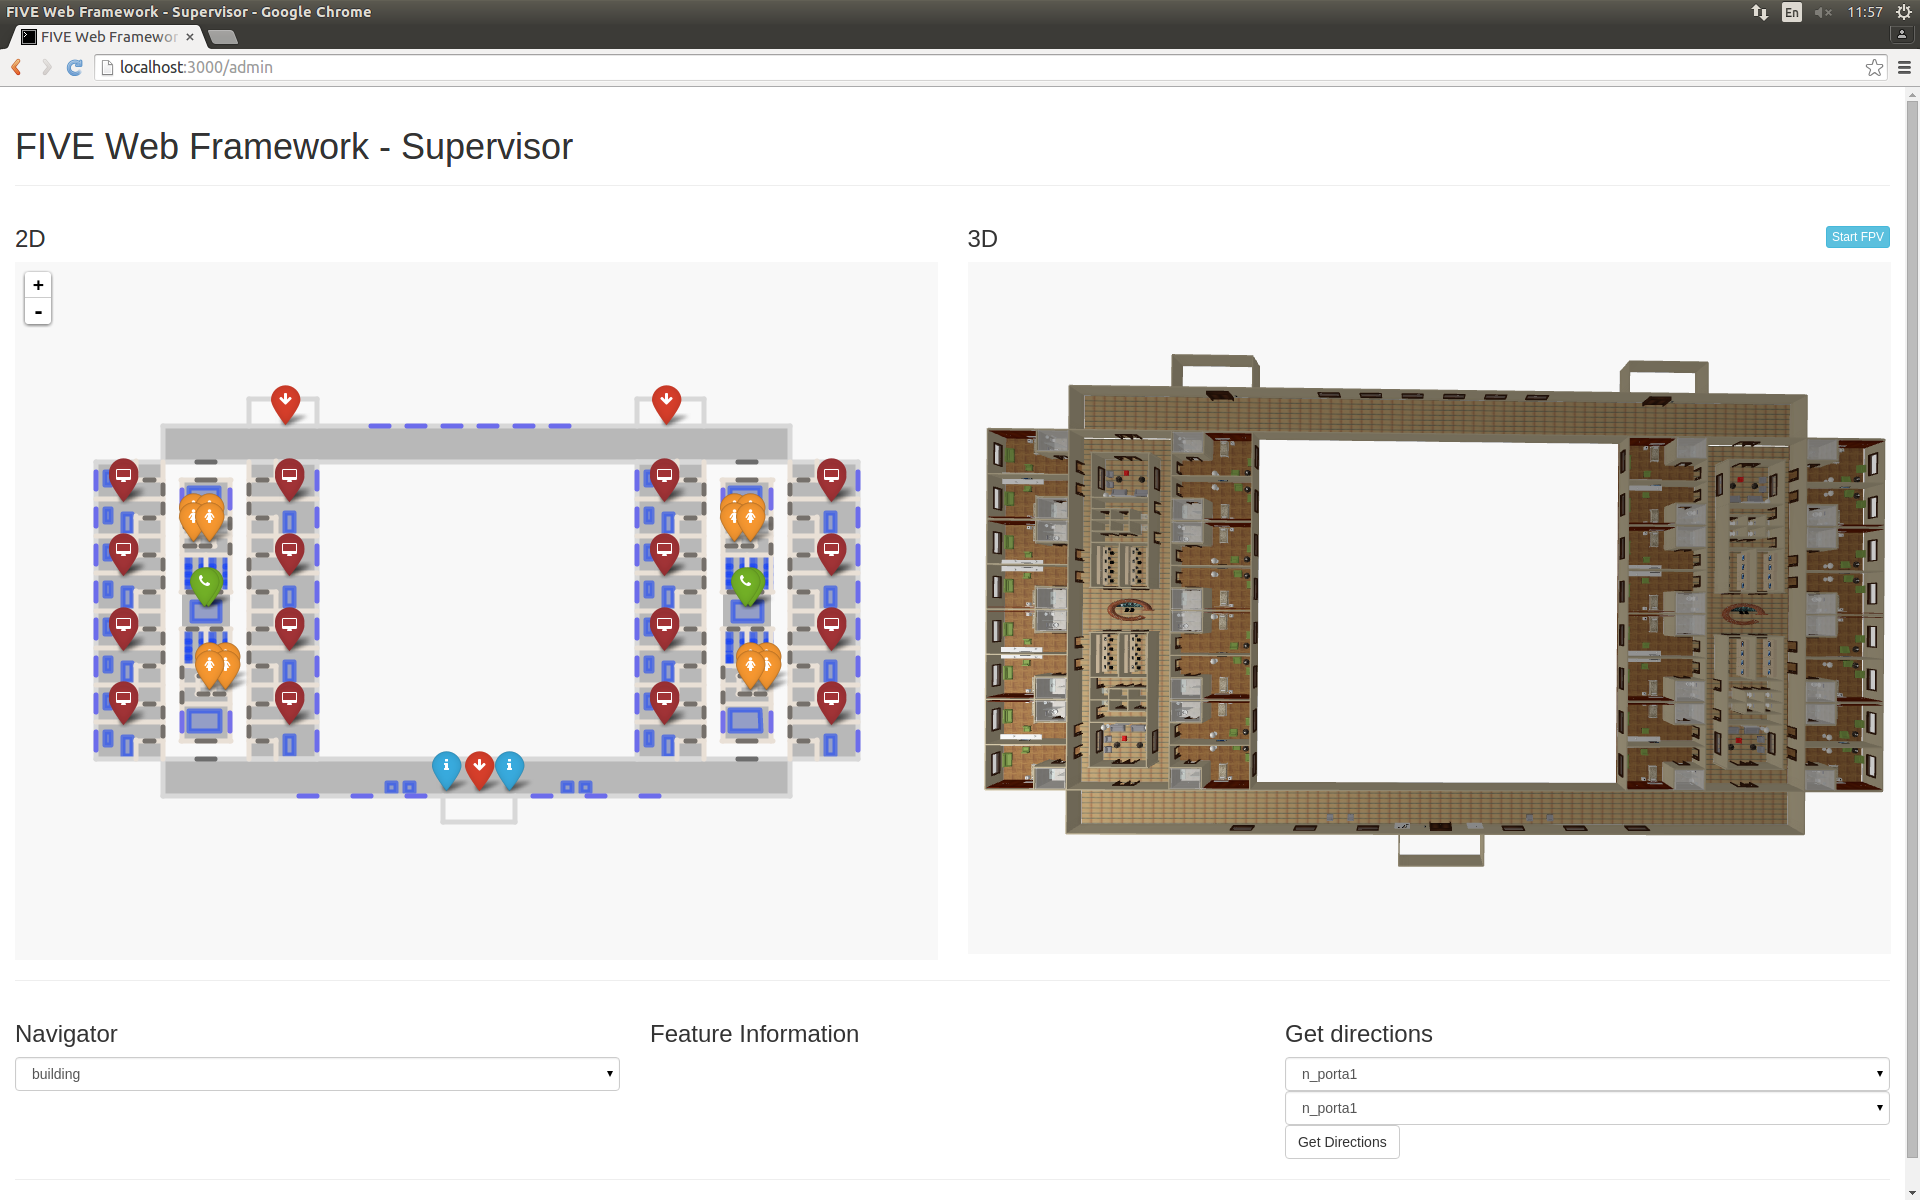
\includegraphics[width=\textwidth]{images/framework-ui.png}
\caption{FIVE Web Framework UI}
\label{fig:web-framework-ui}
\end{figure*}




\emph{GeoJSON} is a geospatial data interchange format based on JSON, suitable for a
geometrical encoding of various geographic data structures. As opposed to GIS
formats, GeoJSON is an open standard. Positions need to be expressed in
geographical coordinates (usually WGS84).

GeoJSON \cite{geojson} allows to define arbitrary objects, called {\tt
Features}, by specifying their {\tt geometry}, and by associtating to them some
{\tt properties}. Complex shapes are defined through the composition of
simple primitive geometric objects. 

Mainly due to its simplicity,
GeoJSON is widely used and deeply integrated into several applications and
services.

\emph{IndoorJSON} \cite{indoorjson} is a GeoJSON variant defined and used by \emph{indoor.io}, a
Finnish company devoted to indoor environment mapping. IndoorJSON is compliant
with GeoJSON syntax, supporting all GeoJSON geometry types.

Customization with respect to GeoJSON format is obtained exploiting particular properties to correctly define the indoor elements: \texttt{level} (which describes which storey contains the feature) and \texttt{geomType} (which identifies the category of the object). A number of non-mandatory indoor properties is also defined: \texttt{accessible} (which describes if an element is walkable or not), \texttt{connector} (which defines if the element is a connection between two
 storeys) \texttt{direction} (which describes the direction of the connection: both
 ways, only up, only down).

A syntax validator is provided by \emph{indoor.io}, but the commercial nature
of this project limits the number of tools available to deal with this
format.
